
\documentclass[12pt]{article}
\usepackage{fullpage,amsmath,amssymb,graphicx}

\usepackage{setspace}
\spacing{1}

\usepackage{textpos}
\usepackage{tikz}
\usepackage{pgf}
\usepackage{amssymb}
\usepackage{enumerate}
\usepackage{xcolor}
\usepackage{graphicx}
\usepackage{subcaption}
\usepackage{tabularx}
\usepackage{colortbl}
\usepackage{multicol}
\usepackage{longtable}
\usepackage{hyperref}
\usepackage{comment}
\usepackage{listings}



\definecolor{encabezado}{rgb}{0.74, 0.83, 0.9}

\begin{document}

\hfill\\
\rule{\textwidth}{1.5pt}

\begin{minipage}[t]{85mm}
  \begin{tabular}{l}
    \textbf{\large Instituto Tecnológico de Costa Rica} \\  
    \textbf{Escuela de Ingeniería Electrónica} \\
    \textbf{Trabajo Final de Graduación} \\
    \textbf{Proyecto:} Método basado en aprendizaje reforzado \\para el control automático de una planta no lineal. \\
    \textbf{Estudiante:} Oscar Andrés Rojas Fonseca \hspace{3cm}\rule{4.5cm}{1.5pt}\\
    I Semestre 2024 \hspace{8.5cm}\textbf{Firma del asesor}
  \end{tabular}
\end{minipage}
\hfill\\
\rule{\textwidth}{1.5pt}


\section*{Bitácora de trabajo}

%\begin{table}[h]
\begin{minipage}[h]{\textwidth}
	\centering
	\begin{tabularx}{\textwidth}{|p{2cm}|X|X|p{2cm}|} 
		\hline
		\rowcolor{encabezado}
		\textbf{Fecha} & 
		\textbf{Actividad} & 
		\textbf{Anotaciones} & 
		\textbf{Horas dedicadas} \\ \hline
		% ***************************************************************
	 	08/04/2024 & 
	 	$\mathbf{1}.$ AAA. & 
	 	$a)$ DDDDDDD \newline & 
	 	6 horas \\
		% ***************************************************************
		09/04/2024 & 
	 	$\mathbf{2}.$ Pruebas de implementación $CUDA$ en Windows. &
	 	$a)$ SASASASAS. \newline & 
	 	4 horas \\
	 	% ***************************************************************
		09/04/2024 & 
	 	$\mathbf{2}.$ Pruebas de entrenamiento del modelo $Pendulum\, DQN$. &
	 	$a)$ SASASASAS. \newline & 
	 	4 horas \\
	 	% ***************************************************************
	 	10/04/2024 & 
	 	$\mathbf{3}.$ Reunión de seguimiento con el asesor del proyecto. & 
	 	$a)$ Revisión de avance en el código y errores de forma.  \newline
	 	$b)$ Dado el factor tiempo para el proyecto y el poco avance realizado, se acordó enfocarse directamente en el env $Pendulum$ de Gymnasium \cite{gym}.  \newline & 
	 	2 horas \\
	 	\hline
	\end{tabularx}
\end{minipage}	 	
	 	
	 	% ***************************************************************
\hfill\\
\begin{minipage}[h]{\textwidth}
	\centering
	\begin{tabularx}{\textwidth}{|p{2cm}|X|X|p{2cm}|} 
		\hline		
		
	 	% ***************************************************************
	 	11/04/2024 & 
	 	$\mathbf{4}.$ Pruebas con entorno $CartPole$ y $Pendulum$ para implementación de CUDA. &
	 	$a)$ Por recomendación del profesor asesor, la implementación se mudó a Ubuntu/Linux para meyor control y referencia. \newline
	 	$b)$ Instalación y creación de nuevos $environments$ mediante la herramienta $micro\, mamba$. \newline & 
	 	5 horas \\
	 	% ***************************************************************
	 	12/04/2024 & 
	 	$\mathbf{5}.$ Revisión del código original para $DQN$ \cite{DQNCart}. &
	 	$a)$ ADADA. \newline & 
	 	4 horas \\
	 	% ***************************************************************
	 	
	 	\hline
		\multicolumn{3}{|r|}{Total de horas de trabajo:} & 21 horas \\ 
	 	\hline                 
	\end{tabularx}
\end{minipage}
%\end{table}



% *****************************************************************************
% *****************************************************************************
% *****************************************************************************

\section*{Contenidos de actividades}

AAA \cite{DQNCart}.

%\begin{figure}[h]
%	\centering
%	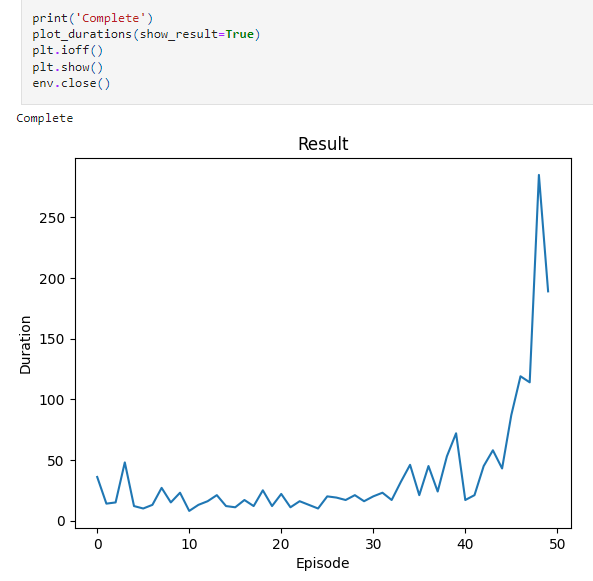
\includegraphics[scale=0.6]{Fig/CapturaCartPole1.png}
%	\caption{Resultado de entrenamiento del modelo para $CartPole$ con $50$ episodios.}
%	\label{fig:Cart1}
%\end{figure}	

\newpage

\section*{Referencias}
\renewcommand\refname{}
\bibliographystyle{IEEEtran}
\bibliography{references}





\end{document}
